\documentclass[accentcolor=tud1c,article,colorback,11pt]{tudreport}
\usepackage[utf8]{inputenc}
\usepackage[ngerman]{babel}
\usepackage[T1]{fontenc}
\usepackage[stable]{footmisc}
\usepackage[ngerman]{hyperref}
\usepackage[ngerman]{cleveref}
\usepackage{longtable}
\usepackage{multirow}
\usepackage{booktabs}
\usepackage{listings}

\newlength{\longtablewidth}
\setlength{\longtablewidth}{0.7\linewidth}
\addtolength{\longtablewidth}{-\marginparsep}
\addtolength{\longtablewidth}{-\marginparwidth}

\uppertitleback{(\textaccent{\textbackslash uppertitleback})}
\lowertitleback{(\textaccent{\textbackslash lowertitleback})\hfill\today}

\hypersetup{
	pdftitle={CTMS Dokumentation},
	pdfauthor={Haixin Cai, Jannik Vieten, Pascal Weisenburger},
	pdfsubject={CTMS Dokumentation},
	pdfview=FitH,
	pdfstartview=FitV
}

\title{CTMS Dokumentation}
\subtitle{Haixin Cai, Jannik Vieten, Pascal Weisenburger}
\subsubtitle{Wintersemester 2013 / 2014}

%\setinstitutionlogo[width]{Hier Institutslogo einfügen!}
\institution{Theoretische Informatik\\Kryptographie und Computeralgebra}
\sponsor{\hfill\includegraphics[height=6ex]{tud_logo}\hspace{1em}}

\begin{document}

\maketitle

\begin{abstract}
Dieses Dokument stellt die Dokumentation zum \textit{CA Trust Management System (CTMS)} dar und gibt Hinweise zur Benutzung sowie zur Architektur der entwickelten Komponenten. Dabei handelt es sich um eine Java-Anwendung die das Trust-Management übernimmt und eine Firefox-Extension, die die CTMS-Funktionalität im Browser benutzbar macht. Die hier vorgestellte Implementierung entstand im Rahmen eines Praktikums bei der CDC-Gruppe des Fachbereichs Informatik an der TU Darmstadt. Programmiert wurde das System von Haixin Cai, Jannik Vieten und Pascal Weisenburger, die Betreuung fand statt durch Johannes Braun und Moritz Horsch.
\end{abstract}
\newpage

\tableofcontents
\newpage

\section{Einleitung}

Die heute im Internet eingesetzte \textit{Public-Key-Infrastruktur (Web-PKI)}, die auf der Integrität von \textit{Certificate Authorities (CAs)} basiert, gerät zunehmend in die Kritik, nicht ausreichend sicher und vertrauenswürdig zu sein. So kann jede CA ein Zertifikat für jede beliebige Domain ausstellen, was Angesichts der Einflussnahme von staatlichen Behörden auf einzelne CAs die Gefahr für Man-in-the-Middle-Angriffe real werden lässt.\\
In \cite{braun2013trust} stellen Braun et~al. ein alternatives Trust-Modell vor, welches dieses Problem adressiert und der Vertrauensentscheidung einen benutzerspezifischen, individuellen \textit{Trust View} zu Grunde legt, der sich den Bedürfnissen des Benutzers anpasst.\\
Dieses \textit{CA Trust Management System (CTMS)} wurde nun implementiert und besteht im Wesentlichen aus zwei Komponenten. Die erste ist eine Java-Anwendung, die das Trust-Management übernimmt, die nötige Funktionalität für das Bewerten von Zertifikaten bereitstellt und sich vom Benutzer konfigurieren lässt. Die andere Komponente wird von einer Firefox-Extension gebildet, die auf die Trust-Berechnung der Java-Anwendung zurückgreifen kann, um während dem Surfen im Internet die Nutzung des CTMS möglich zu machen.

\section{CTMS-Anwendung}

Im Folgenden wird das CTMS-System beschrieben.

\subsection{Entwicklungsumgebung}
Die Anwendung baut auf Java 7 auf. Da zur Entwicklung Eclipse genutzt wurde, liegt ein Eclipse-Projekt vor. Die gesamte Anwendung lässt sich aber auch mit Hilfe einer Ant-Build-Datei kompilieren. Die dabei generierte \texttt{JAR}-Datei enthält alle nötigen Abhängigkeiten. Dabei handelt es sich um die folgenden Bibliotheken:
\begin{description}
\item[CertainTrust SDK (CertainTrustSDK-1.0.jar)] ist das grundlegende Toolkit zur Modellierung/Berechnung von Computational Trust
\item[Java JSON API (javax.json-1.0.4.jar)] wird benötigt um eingehende Validierungsanfragen (von der Firefox-Extension) zu lesen, die in JSON kodiert sind
\item[Java JDBC connection pool manager (miniconnectionpoolmanager.jar)] ist ein einfacher Manager, um JDBC-Datenbankverbindungen zu verwalten
\item[SQLite connection pool (sqlite-connection-pool\_v1.1.0.jar)] stellt einen Pool für SQLite-Verbindungen zur Verfügung, der im Zusammenspiel mit dem \textit{Java JDBC connection pool manager} genutzt wird, um einen Pool von wiederverwendbaren und potentiell nebenläufigen SQLite-Verbindungen zu verwalten
\item[SQLite JDBC (sqlite-jdbc-3.7.2.jar)] stellt den Zugriff auf SQLite-Datenbanken zur Verfügung, der zur persistenten Daten-Speicherung genutzt wird
\item[Notary module (sslcheck-1.0-jar-with-dependencies.jar)] stellt das Modul zur Abfrage von Notaries zur Verfügung
\end{description}

\subsection{Überblick}
Das System besteht im Wesentlichen aus
\begin{itemize}
\item dem Datenmodell zur Verwaltung des \textit{Trust Views} und der Benutzerkonfiguration
\item der Trust-Validierung zur Berechnung der Vertrauenswerte im Trust-Modell
\item Bindings zur Kommunikation mit Anwendungen, damit diese das Trust-Modell benutzen können
\item einer graphischen Oberfläche, mit deren Hilfe der Benutzer den Trust View  einsehen und verwalten kann
\end{itemize}
\Cref{overview} bietet einen Überblick über diese Komponenten und deren Interaktion.

\begin{figure}[h]
  \centering
  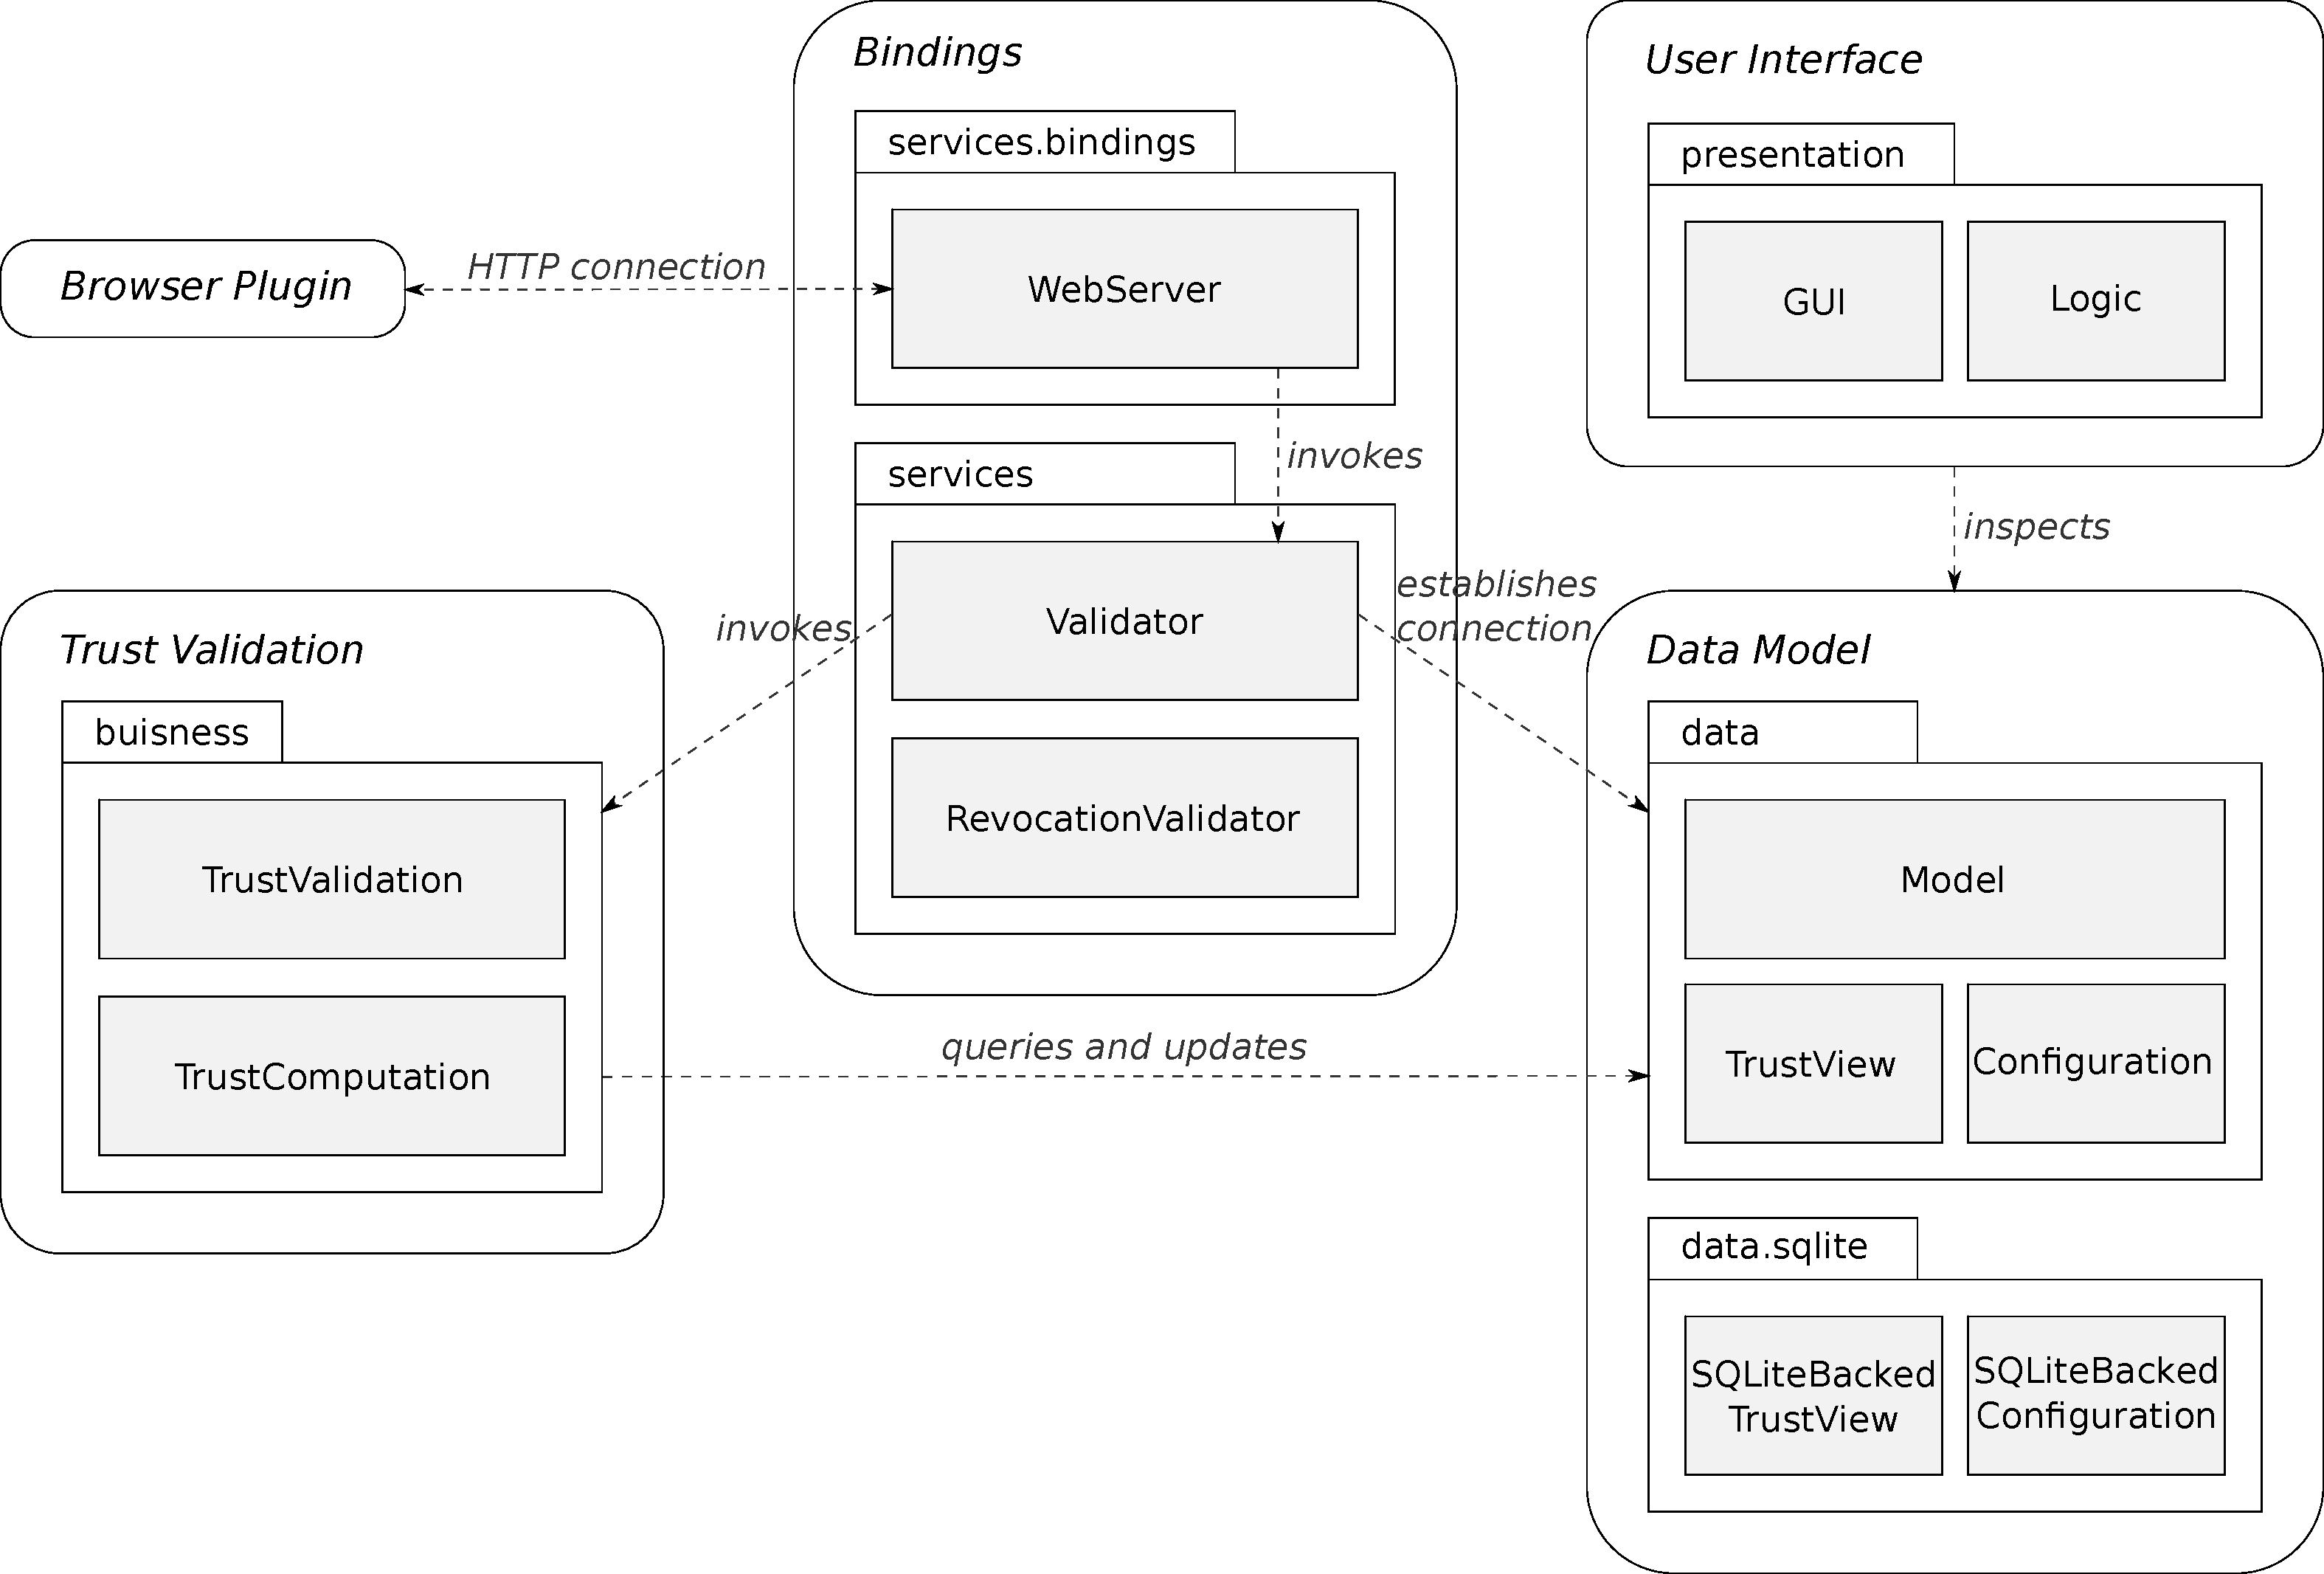
\includegraphics[width=\textwidth]{overview}
  \caption{Überblick über die Komponenten des CA Trust Management Systems}
  \label{overview}
\end{figure}

\subsection{Datenmodell}
Das Datenmodell verwaltet den Trust View, in dem die \textit{Public Key Trust Assessments} und die Menge vertrauenswürdiger und nicht vertrauenswürdiger Zertifikate gespeichert sind, wie in \cite{braun2013trust}, Abschnitt 4.2 beschrieben.

Darüber hinaus stellt das Datenmodell den Zugriff auf die Benutzerkonfiguration zur Verfügung. Standardwerte sind in der Datei \texttt{configuration.properties} im Wurzelverzeichnis der Applikation/\texttt{JAR}-Datei festgelegt und können dort modifiziert werden. Vom Benutzer angepasste Werte werden von der zugrunde liegenden Implementierung des Modells an einem benutzerspezifischem Ort gespeichert, wie dies auch mit dem Trust View geschieht.

Die momentane Implementierung des Modells in den Klassen \texttt{data.sqlite.SQLiteBackedTrustView} und \texttt{data.sqlite.SQLiteBackedConfiguration} nutzt eine SQLite-Datenbank zum Speichern der Daten. Die Datenbank-Datei \texttt{ctms.sqlite} wird abgelegt im Verzeichnis:

\vspace{1em}
\begin{minipage}{\textwidth}
\begin{description}
\item[Windows] \%APPDATA\%\textbackslash ctms
\item[OS X] \textasciitilde/Library/Application Support/ctms
\item[andere (falls \$XDG\_DATA\_HOME gesetzt)] \$XDG\_DATA\_HOME/ctms
\item[andere (falls \$XDG\_DATA\_HOME nicht gesetzt)] \textasciitilde/.local/share/ctms
\end{description}
\end{minipage}
\vspace{1em}

Die Implementierung des Datenmodells kann ggf. einfach gegen eine andere ausgetauscht werden. Dazu muss lediglich die Klasse \texttt{data.Model} angepasst werden, sodass eine andere Implementierung genutzt wird, welche Realisierungen der Interfaces \texttt{data.TrustView} und \texttt{data.Configuration} bereitstellt.

Zentraler Zugriff auf das Datenmodell erfolgt über die Klasse \texttt{data.Model}. Über die Methoden \texttt{openTrustView} und \texttt{openConfiguration} können Instanzen der Interfaces \texttt{TrustView} bzw. \texttt{Configuration} geöffnet werden. Nach dem Ende der Transaktion also dem Abfragen und Aktualisieren des Datenmodells, müssen die geöffneten Instanzen wieder geschlossen werden. Es ist dabei sicher gestellt, dass die Transaktion atomar ist, sie also komplett ausgeführt oder komplett nicht ausgeführt wird und die Daten somit konsistent bleiben.

\subsection{Trust-Validierung}

Die Algorithmen zur Berechnung der Trust-Werte und zur Trust-Validierung sind in der Klasse \texttt{buisness.Computation} implementiert. Es handelt sich dabei um die in \cite{braun2013trust}, Abschnitte 4.3, 4.4 und 4.5 beschriebenen Algorithmen der Initialisierung der Trust Assessments, der Trust-Validierung und der Trust-View-Aktualisierung.

Die Standardpfadvalidierung wird von Firefox ausgeführt und das Resultat wird der Java-Applikation übermittelt. Diese prüft die Gültigkeit/Revokation der Zertifikate und die Gültigkeit des Zertifikatspfades nicht mehr selbst, sondern verlässt sich auf die Validierung, die von Firefox ausgeführt wurde. Dies bedeutet insbesondere auch, dass für die Gültigkeit der Root Certificate Store von Firefox maßgeblich ist und nicht der der Java Runtime. Die Klassen im Package \texttt{support.revocation} sind deshalb zurzeit nicht implementiert.

\subsection{Bindings}
Bindings stellen eine Schnittstelle für andere Anwendungen zur Verfügung, um das Trust-Modell nutzen zu können. Die allgemeine Funktionalität, die von allen Bindings genutzt werden kann, wie der Zugriff auf die Trust-Berechnung-Komponente und das Datenmodell, um die Trust-Validierung auf dessen Basis auszuführen, ist in der Klasse \texttt{services.logic.Validator} implementiert. Momentan existiert ein Binding \texttt{services.bindings.WebServer}, das einen simplen WebServer zur Verfügung stellt, über den das ebenfalls im Rahmen dieses Projektes entwickelte Firefox-Plugin mit dem CTMS kommunizieren kann, um den Service der Trust-Validierung zu nutzen. Der Webserver kann über die graphische Oberfläche gestartet werden.

\subsection{Graphische Oberfläche}
Das CTMS kann über die grafische Benutzeroberfläche gesteuert werden, die sich in \texttt{presentation.ui} befindet. Wichtigste Funktion ist das Starten des Webservers, über den die Firefox-Extension mit der Java-Anwendung kommunizieren kann. Außerdem ist das Ansehen und Bearbeiten von vertrauenswürdigen und unvertrauenswürdigen Zertifikaten sowie den \textit{Trust Assessments} möglich. In der Konfigurationsansicht können die Werte für die Security-Level und den TCP Port angepasst werden. Zudem ist es möglich, die Datenbank, in der der Trust View gespeichert ist, zu löschen oder ein Backup zu erstellen bzw. wieder einzuspielen. Die Nutzung des Notary-Moduls ist freiwillig und kann, insbesondere zu Testzwecken, mit einem gewünschten Ergebnis überschrieben werden. Dafür bietet die grafische Oberfläche eine Einstellungsmöglichkeit.

\section{Firefox-Extension}
Im Folgenden wird die zum CTMS-System gehörige Firefox-Extension beschrieben.

\subsection{Überblick}
Standardmäßig akzeptiert Firefox alle gültigen Zertifikate, die von beliebigen, im Browser registrierten CAs ausgestellt wurden. Das sind inzwischen sehr viele und diese Tatsache liegt dem Vertrauens-Problem der derzeitigen Web-PKI zu Grunde. Um das alternative Vertrauenskonzept der Trust Views zu benutzen, integriert sich die Firefox-Extension in den Browser und delegiert die Trust-Berechnung an die CTMS-Anwendung, um anschließend angemessen auf das Ergebnis zu reagieren und den Benutzer ggf. zu warnen.

\subsection{Installation}
Die Installation der Extension funktioniert wie von Firefox-Addons gewohnt. Liegt keine fertige .xpi-Datei vor, muss diese zunächst erzeugt werden. Dazu wird der Inhalt des Ordners, der die Extension enthält, in ein zip-Archiv gepackt. Die Dateiendung sollte anschließend in .xpi geändert werden. Es sollte nun also eine Datei \texttt{trustviewsextension@cdc.informatik.tu-darmstadt.de.xpi} existieren, in der sich auf oberster Ebene (unter anderem) die Datei \texttt{install.rdf} befindet. Die .xpi Datei kann dann in den Firefox gezogen werden und wird folglich installiert.

\subsection{Benutzung}
Während der Installation der Extension wird ein zusätzlicher Button in die Toolbar des Browsers integriert. Über diesen Button wird ein Menü bereitgestellt, in dem Einstellungen vorgenommen werden können. Dort lässt sich das Sicherheitslevel auf eine der drei Stufen \glqq hoch\grqq, \glqq mittel\grqq ~oder \glqq niedrig\grqq ~einstellen, was das Sicherheitsbedürfnis des Benutzers für die Webseiten widerspiegeln soll, die als nächstes besucht werden. Für Online-Banking oder e-Commerce dürfte beispielsweise ein höheres Level erforderlich sein, als für das Lesen einer Nachrichtenseite. Das ausgewählte Sicherheitslevel geht dann als Parameter in die Vertrauensberechnung der CTMS-Anwendung ein. Außerdem lässt sich über das Menü das Konfigurationsfenster der Extension aufrufen, in dem die Verbindungsinformationen (Host und Port) zur CTMS-Anwendung geändert werden können, mit der die Extension über HTTP kommuniziert.\\
Wird eine mit TLS geschützte Seite aufgerufen, nimmt die Extension Kontakt mit der CTMS-Anwendung auf und erwartet von ihr das Urteil, ob die Seite bzw. das ausgelieferte Zertifikat vertrauenswürdig ist. Ist das nicht der Fall, wird der Benutzer auf eine Warnseite umgeleitet, die den Sachverhalt erklärt, dem Benutzer aber gleichzeitig die Möglichkeit gibt es mit geändertem Sicherheitslevel erneut zu versuchen, oder die Website in jedem Fall zu besuchen. Bei letzterer Möglichkeit wird die betroffene Website für die Dauer der Browsersitzung von weiteren Trust-Überprüfungen ausgenommen.\\
Ist die CTMS-Anwendung nicht erreichbar, wird ebenfalls eine Warnseite angezeigt, die den Benutzer dazu auffordert die CTMS-Anwendung zu starten oder die Extension zu deaktivieren.

\subsection{Architektur}
Im Folgenden wird auf die einzelnen Komponenten der Extension eingegangen und die ihr zugrunde liegende Architektur beschrieben.

\subsubsection{Namespace}
Um Namenskonflikte bei der Wahl von Bezeichnern wie Funktionsnamen zu vermeiden, befinden sich alle zur CTMS-Extension gehörigen JavaScript-Objekte innerhalb des Namespace \texttt{TVE} (kurz für Trust-Views-Extension). Beispiele hierfür sind die Objekte \texttt{TVE.SSLListener} und \texttt{TVE.UI}. In den folgenden Beschreibungen wird das Präfix TVE meist weggelassen.\\
Der Namespace wird innerhalb der Datei \texttt{setupNamespace.jsm} angelegt, der als JavaScript-Modul \cite{jsm} geschrieben wurde, s.~d. es keine Probleme mit dem Scoping über mehrere XUL-Seiten hinweg gibt. Außerdem wird beim Setup auch der entsprechende Preferences-Branch and den Namespace gebunden.

\subsubsection{Initiierung}
Nachdem der Namespace erzeugt und alle nötigen Skripte geladen wurden, wird die Datei \texttt{init.js} ausgeführt. Dort wird das Objekt \texttt{SSLListener} als WebProgressListener registriert um über HTTPS-Seitenaufrufe informiert zu werden. Diese Registrierung muss jedoch durch die Methode \texttt{addTabsProgressListener()} \cite{allTabs} erfolgen, um auch mit mehreren Tabs zu funktionieren.\\
Wird \texttt{init.js} das erste Mal nach der Installation ausgeführt, werden noch zusätzliche Schritte unternommen um die Extension für die erste Benutzung vorzubereiten. Dazu wird der Button der Extension zur Toolbar von Firefox hinzugefügt und das Security-Level wird auf \glqq mittel\grqq~ eingestellt. Die wesentliche XUL-Datei bis zu diesem Punkt ist \texttt{browserOverlay.xul}.

\subsubsection{SSLListener}
In der Datei \texttt{sslListener.js} befindet sich das Objekt \texttt{SSLListener}, welches bereits von \texttt{init.js} als WebProgressListener \cite{progressListener} registriert wurde. \texttt{SSLListener} wird aktiv, wenn eine neue HTTPS-Verbindung aufgebaut wird und regelt dann das weitere Vorgehen der Extension. Das CTMS wird nur kontaktiert, wenn Firefox/NSS die Zertifikatskette erfolgreich validieren konnte. Für die weitere Validierung durch das CTMS werden neben der URL und dem Validierungsergebnis von Firefox/NSS das vom Benutzer gesetzte Security-Level und die Zertifikatskette benötigt. Letztere wird vom \texttt{CertHandler} ausgelesen. Die Kommunikation mit dem CTMS wird dann vom \texttt{CTMSCommunicator} durchgeführt, der entsprechende Callback-Funktionen im \texttt{SSLListener} aufruft, um das Ergebnis der Validierung verfügbar zu machen. Dieses Ergebnis ist entweder \glqq TRUSTED\grqq, \glqq UNKNOWN\grqq~oder \glqq UNTRUSTED\grqq. In letzterem Fall wird das \texttt{State} Objekt angewiesen eine Warnseite anzuzeigen. Schlägt die Kommunikation mit dem CTMS fehl, etwa weil der Webservice nicht erreichbar ist, wird stattdessen eine entsprechende Fehlerseite angezeigt.

\subsubsection{Certificate Handler}
Der \texttt{CertHandler} aus der Datei \texttt{certHandler.js} stellt eine Funktion bereit, um die Zertifikatskette der aktuellen Verbindung auszulesen. Zurückgegeben wird dabei ein Array, welches alle Zertifikate der Kette enthält. Jeder Eintrag ist wiederum ein Bytearray welches ein Zertifikat im DER-Format \cite{DER} repräsentiert. Das erste Zertifikat im Array ist das der Root-CA, das letzte Zertifikat das des Servers.

\subsubsection{Kommunikation mit dem CTMS}
In \texttt{ctmsCommunicator.js} ist das Objekt \texttt{CTMSCommunicator} definiert, welches Validierungsanfragen an die CTMS-Anwendung stellen kann. Kommuniziert wird dabei über HTTP. Der \texttt{CTMSCommunicator} packt die erforderlichen Parameter (URL, Zertifikatskette, Standardvalidierungsergebnis und Security-Level) in ein JSON-codiertes Objekt und verschickt dieses per HTTP-POST mittels eines \texttt{XMLHttpRequest} \cite{httpRequest}. Außerdem werden die \texttt{onload} und \texttt{onerror} Callback-Funktionen gesetzt, über die der aufrufende \texttt{SSLListener} vom Ergebnis erfährt.

\subsubsection{State}
Das in \texttt{state.js} definierte Objekt \texttt{State} ist dafür zuständig Warnseiten anzuzeigen, sowie eine Liste temporär erlaubter Seiten zu managen, die während der aktiven Sitzung von der Trust-Überprüfung ausgenommen werden.\\
Schlägt der Verbindungsaufbau mit dem CTMS fehl, wird die Warnseite \texttt{ctmsUnreachable.xul} angezeigt, auf der dem Benutzer erklärt wird, dass der Webservice aktiviert werden sollte.\\
Wird hingegen ein Zertifikat für unvertrauenswürdig erachtet, wird der Benutzer auf der Warnseite \texttt{untrustedWebsite.xul} gewarnt und erhält die Möglichkeit, es mit geändertem Sicherheitslevel erneut zu versuchen, oder die Warnung zu ignorieren und die Website dennoch zu besuchen. In letzterem Fall wird die entsprechende Seite für die aktive Sitzung von Trust-Überprüfungen ausgenommen.

\subsubsection{Optionen} 
In \texttt{options.xul} ist ein Einstellungsfenster definiert, in dem sich die Verbindungsinformationen zum CTMS verändern lassen. Es ist möglich, die Einstellungen auf die Standardwerte zurückzusetzen. Diese Funktionalität stellt das \texttt{UI} Objekt aus \texttt{ui.js} bereit.

\newpage
\bibliographystyle{plain}
\bibliography{references}

\end{document}
